\documentclass[12 pt]{scrartcl}
\usepackage{setspace}
\onehalfspacing
\usepackage{amsmath,amssymb,amsfonts,amsthm,mathtools}
\usepackage[english]{babel}
\usepackage[T1]{fontenc}
\usepackage[utf8x]{inputenc}
\usepackage{lmodern}
\usepackage{dsfont}
\usepackage{bbm}
\usepackage[round]{natbib}
\usepackage{color} 
\usepackage[defaultlines=2,all]{nowidow}
\usepackage{caption}
\usepackage[labelformat=simple]{subcaption}
\usepackage{makecell}
\renewcommand\thesubfigure{(\alph{subfigure})}

\setlength\parindent{0pt}
\setlength{\parskip}{6pt plus 1pt minus 1pt}

\newcommand{\red}{\textcolor{red}}


\begin{document}

\begin{titlepage}
  \centering
  {\scshape\LARGE TU Dortmund \par}
  \vspace{1cm}
  {\scshape\Large Introductory Case Studies \par}
  \vspace{2cm}
  {\huge\bfseries Project 2: Comparison of rental prices in the Ruhr area\par}
  \vspace{2cm}
  {\Large Lecturers:\\
    Prof.\ Dr.\ Sonja Kuhnt\\
    Dr.\ Paul Wiemann\\
    Dr.\ Birte Hellwig\\
    M.\ Sc.\ Hendrik Dohme \par}
  \vspace{1cm}
  {\Large Author: Tadeo Hepperle \par}
  \vspace{0.5 cm}
  {\Large Group number: 28\par}
  \vspace{0.5 cm}
  {\Large Group members: Dhanya Zacharias, Imene Kolli, Vanlal Peka, Sara Zhara, Tadeo Hepperle}
  \vfill
  {\large \today\par}
\end{titlepage}


\tableofcontents

\cleardoublepage

\section{Introduction}

Everyone needs to have a place to live. That is why rent and housing prices affect almost everyone and play a huge role in ones life. Data suggests, that the average German spends 28 percent of their income on rent which is about 720 euros per month \citep{statistarent}. This makes local rental prices an important factor in deciding where to live, especially since rental prices have been increasing year after year since 1997 \citep{deutschlandinzahlen}.
In this project we will take a look at rental prices in the 4 largest cities of the ruhr area (Dortmund, Duisburg, Bochum and Essen) and analyze whether or not rental prices differ between those regions. For this, data from the web platform Immobilienscout24 was taken. Immobilienscout24 brings landlords and real estate firms together with potential tenants and provides transparency in terms of prices. For each of the 4 cities, 50 properties were sampled.
The average rent across cities is 9.15 €/m² with a standard deviation of 1.29 €/m².
An Analysis of Variance (ANOVA) was run on this data, to see if any of the cities differ in the mean reantal price. There was a significant effect, indicating that the rental price is not the same across all 4 cities.
After that, we conducted 6 bonferroni-corrected two group ANOVAs for all possible pairs of cities, to find out if there are significant differences between the rental price of two designated places. This yielded the result, that the rent per square meter in Duisburg is significantly lower than in Dortmund and Essen. Other than that the effects were too small to become significant.
First, in Section 3 an overview is given on how the data was collected and its quality is asessed. Also we present the goals of the project. In Section 3 the statistical and computational methods will be discussed, in particular the concept of hypothesis testing and how an Analysis of Variance works.
Section 4 displays the data analysis results, where we find out which differences in rental prices between cities turned out to be significant. Finally Section 5 gives a brief summary and highlights potential implications of the findings for people that might want to rent a property in the Ruhr area.

\section{Problem statement}

We analyzed a dataset containing the rental prices of 200 properties in the Ruhr area to find out if there are differences in the mean rental prices between Dortmund, Duisburg, Bochum and Essen.

\subsection{Description of the dataset}

The data used in our analysis is a subset of a dataset from \citet{kaggle}. It was originally scraped from www.Immobilienscout24.de, an online real estate marketplace on February 20, 2020. Immobilienscout24 belonging to the Scout24 AG had a revenue of 353.5 million dollars in 2020 and is one of the largest real estate online marketplaces in germany \citep{statista}.
The dataset consists of rental prices for 200 properties in the Ruhr area. The data was randomly sampled in such a way that we have exactly 50 properties for each of the large cities Dortmund, Bochum, Duisburg and Essen. The respective city is the indepentent variable in the context of this study. The rental price in euros per square meter resembles a metric depentant variable. The data was gathered in a purely observational way, which introduces a couple of biases. First of all we do not know if prices from Immobilienscout24 are representative for the entire market. For example it could be, that there is a portion of rental contracts that have been running for years or decades and therefore may have lower rent then newly issued contracts. Increasing Rent is a common occurance when tentants change. Also we do not know anything about the type of properties and the position with respect to the city center. We can just assume the random sampling kept those factors somewhat constant for all 4 cities, even though we do not even know if the original dataset our sample comes from may have been biased in the first place. In Addition to that it is unknown to us how balconies, roof slopes and gardens have been factored into the calculation of the rental price in Euros per square meter.
The rental price relates to the net rent: service charges come on top of that. Unfortunately we cannot even make the assumption that net rent and service charges are independent from each other, as it is common practice to advertise a property by stating a lower net rent while inscresing certain service charges.
There is no missing data, but having just 50 objects per group is not a lot. The randomness of the sampling alone can be responsible for some variation between the groups.
Therefore the quality of the dataset is quite weak and the results should not be overinterpreted. Despite that, the averages over the 50 properties for each city should make a rough estimation quite possible.

\subsection{Objectives of the report}

The main objective of the report is, to find out if the mean rental price differes between the 4 cities Dortmund, Bochum, Duisburg and Essen. For this we conduct an ANOVA which yields if there are any significant differences at all, but does not tell, between which cities they are. The Anova is basically asking if a substantial amount of variance in the data can be linked to differences in the means of the 4 groups.
After this we want to figure out, if any pair of cities has a significant difference in their mean rental prices. For those pairwise comparisons we also run an ANOVA with just the two data vectors of the resepctive two cities involved. The alpha level for those two group anovas is bonferroni corrected to not accumulate an alpha error.
With this report we hope to find out if the differences in the data just come from random variation or can be actually linked to the city as a factor. This could in turn help people make decisions about moving and provide a better understanding of the real estate market in the Ruhr area.

\section{Statistical Methods}

First a brief overview of hypothesis testing as a method for finding significant effects is presented. After that the used testing-methods and how to check their requirements is explained.

\subsection{The concept of hypothesis testing}

A lot of times we want to use gathered data to infer a distribution of the underlying distribution the data was taken from. The problem is, that our sample is just a random fraction of the population and therefore statistics like mean and standard deviation might differ from the true parameters one would be able to observe if the entire population was known.
To adress this problem hypothesis testing is used. The basic idea is, that we have a null hypothesis ($H_0$) and an alternative hypothesis ($H_1$). They are mutually exclusive \citep[p.~218]{eid2017statistik}.
For example a null hypothesis ($H_0$) could be that the mean of a population is equal to 10. Then the alternative hypothesis ($H_1$) is that the mean is unequal to zero.
\[ H_0: \mu = 10  \ \ \ \ \ \   H_1: \mu \neq 10 \]

Now some standardized rules need to be introduced, to decide if a sample is probably from a population where $H_0$ holds ($H_0$ gets accepted), or if it is more likely that $H_1$ reflects the real population ($H_0$ gets rejected). For this a Test statistic $T$ is calculated from the data. Also we decide a value for $\alpha$, usually $\alpha = 0.05$ is chosen.
Now we say that we reject the null hypothesis, if it would be very unlikely to observe data with statistic $T$ if $H_0$ was true. In Detail: We reject $H_0$ if the probability of observing $T$ or an even extreme value is less or equal to $\alpha$ under the assumtion that $H_0$ is true. To calculate this probability some distribution of $T$ is assumed for the case that $H_0$ is true, depending on what kind of statistic $T$ is used. So $\alpha$ is the probability of committing a type I error if $H_0$ is true. That is rejecting the null hypothesis, even though it is correct \citep[p.~222]{eid2017statistik}. Conversely the mistake of not rejecting the null hypothesis, even though it is not correct is called type II error.
The probability of observing a value of $T$ or an even more extreme one under the assumtion that $H_0$ is true is called $p-value$.
The range of values for $T$ where $H_0$ is rejected is the rejection region. A value for the test statistic that lies right on the border of the rejection region is called critical value or $T_{crit}$. Comparing $T_{crit}$ with the actual $T$ of the data, provides a means of rejecting or accepting $H_0$: If $T$ is more extreme than $T_{crit}$ the null hypothesis is rejected.
The entire process of hypothesis testing can be summarized by 4 steps:
\begin{enumerate}
  \item Define $H_0$, $H_1$ and $\alpha$.
  \item Define how the test statistic $T$ will be calculated, and derive the rejection region and $T_{crit}$ from the assumed distribution of $T$ under the assumption that $H_0$ holds.
  \item Collect data and calculate $T$ from the sample.
  \item Reject or Accept $H_0$ based on $T$ and $T_{crit}$.
\end{enumerate}
Another way of telling whether or not to reject $H_0$ is by comparing the $p-value$ to $\alpha$: if $p \leq \alpha$ $H_0$ shall be rejected, as in this case $T$ is more extreme than $T_{crit}$.


\subsection{One-way ANOVA}

A one-way ANOVA (short for: One-way analysis of variance) is a statistical test that is used to determine if there are differences between the means of $k$ samples.
For this the Variance of the samples is decomposed, hence the name \citep[p.~392]{eid2017statistik}.
A one-way ANOVA for independent groups requires a metric random variable X and $n = \sum^{k}_{j=1} n_{j}$ realizations. Those belong to k distinct groups, where $n_{j}$ denotes the number of datapoints in group j. The null hypothesis of an ANOVA is, that all k groups have the same mean in their underlying populations, while the alternative hypothesis states that at least one pair of groups do not have the same mean. No direction is specified here.
\[ H_0: \forall i,j \in \{1,...,k\}: \ \mu_{i} = \mu_{j}  \ \ \ \ \ \ \ \   H_1: \exists i,j \in \{1,...,k\}: \ \mu_{i} \neq \mu_{j}  \]
Now, three different square sums can be defined, $SS_{within}$, $SS_{between}$ and $SS_{total}$ such that $SS_{within} + SS_{between} = SS_{total}$ \citep[p.~397]{eid2017statistik}. Here $x_{mj}$ is the m-th datapoint of the k-th group, $\overline{x}$ represents the mean of all datapoints and $\overline{x}_j$ is the mean of all datapoints from group j:
\[ SS_{total} = \sum^{k}_{j=1} \sum^{n_j}_{m=1} ( x_{mj} - \overline{x} )^2 \]
\[ SS_{within} = \sum^{k}_{j=1} \sum^{n_j}_{m=1} ( x_{mj} - \overline{x}_j )^2 \]
\[ SS_{between} = \sum^{k}_{j=1} \sum^{n_j}_{m=1} ( \overline{x}_j - \overline{x} )^2 \]
The idea is that, in case there are substantial differences between the group means, the $SS_{between}$ will be larger in relation to $SS_{within}$, than if the group means would be the same and differences stem only from random variation. Therefore the test statistic F has to reflect this relationship. First mean square sums $MSS_{within}$ and $MSS_{between}$ are calculated from $SS_{within}$ and $SS_{between}$ \citep[p.~397]{eid2017statistik}. For the following we assume equal sample sizes:
\[ MSS_{within} = \frac{SS_{within}}{n-k} \]
\[ MSS_{between} = \frac{SS_{between}}{k-1} \]
Then the resulting test statistic F can be calculated. A larger F signifies that there are differences in the means of the groups.
\[ F = \frac{MSS_{between}}{MSS_{within}} \]
This F statistic follows an $F(df_{1},df_{2})$ distribution with $df_{1} = df_{between} = k-1$ and $df_{2} = df_{within} = n - k$ degrees of freedom, in case the null hypothesis is true.
Therefore we can calculate the critical value $F_{crit}$ as the $1-\alpha$-percentile of the $F(df_{between},df_{within})$ distribution and compare it to our actual F-value received from the sample data. $H_0$ is accepted if $F \leq F_{crit}$.
To run an Anova correctly a few requirements have to be fullfilled.
First of all the values in each group have to be independent and randomly drawn from a population \citep[p.~401]{eid2017statistik}. Also they have to be normally distributed within each group and the variance within the groups should be aproximately equal.
When an ANOVA is conducted for 2 groups only and equal variance of the groups is assumed, it's decision is equal to a two sample t-Test for independent samples. Therefore an Anova can also be used to determine if a difference between just two groups is significant or not.

\subsection{Q-Q plot}

A Q-Q plot (abbreviated from Quantile-Quantile plot) can be used to compare the distribution of a sample with a theoretically assumed distribution \citep[p.~97]{eckstein2006angewandte}. It consists of two perpendicular axis. For every quantile q from a fixed number of evenly distributed quantiles (for example $(q)-quantiles for q \in \{0,0.01,0.02,1\} $) a point is plotted at the position (x,y) in the plot, where y is the q-quantile of the values in the observed sample and x is the q-quantile of the assumed distribution. If the values follow a relatively staright line, the assumed distribution matches the distribution of the sample data very well.
When checking for a normal distribution, the sample data may be z-standardized before fed into the plot, because in this way both axis are in the same scale.
Figure ~\ref{fig:qqplots} shows a Q-Q plot later in this report.

\subsection{bonferroni correction}

As described earlier, statistical testing holds the risk of making a type I error, also called $\alpha$-error, which happens if the null hypothesis is actually true, but by random variation the sample statistic is so extreme, that it falls into the rejection region. As we set the $\alpha$-level delibirately we can control the chance of making this error. But as we increase alpha we reduce the chance of discovering an actual effect at the same time. $\alpha = 0.05$ has been proposed as a universally acceptable $\alpha$-level \citep[p.~219]{eid2017statistik}. One can now imagine that even though the chance of making an $\alpha$-error does not exceed $\alpha$ for a single test, if we conduct multiple statistical tests, the chance of making an $\alpha$-error in at least one of them accumulates as the number of tests increases \citep[p.~416]{eid2017statistik}.
To adress this issue when conducting m tests, we can define a family-wise-alpha $\alpha_{fam}$ and set it to $0.05$. Now we can specify that we want to keep the probability to make an $\alpha$-error in any of the m tests, below $\alpha_{fam}$. To achieve this, the bonferroni-correction suggests to correct the $\alpha$-level of every individual test to $\alpha_{r} = \frac{\alpha_{fam}}{m}$ \citep[p.~417]{eid2017statistik}
So the more tests are conducted in parallel, the stricter $\alpha_{r}$ is chosen for each test, keeping the family-wise-alpha $\alpha_{fam}$ at a constant level independent from the number of tests.

\section{Results}

For the rental price data set, first a few descriptive statistics are provided, before the requirements of the statistical tests are checked and said tests are conducted to find differences in the mean rental price between the four cities Dortmund, Bochum, Duisburg and Essen.

\subsection{Descriptive Statistics}

As Table \ref{tab:descriptives} shows, the average rental price per m² is 9.15 € across the 4 cities and varies by less than 11 percent between any two cities.
Dortmund is the city with the greatest average and median rent (9.15 €/m² and 9.18 €/m²) while both values are lowest in Duisburg (8.62 €/m² and 8.66 €/m²). The standard deviation of 1.29 € across the entire dataset shows that the rental price has relatively low variation. Mean and Median prices are very proximate in all cities which is an indication of a quite symmetrical distribution around the mean.

\begin{table}[ht]
  \centering
  \captionabove{Rental prices in in €/m²: Mean, median, standard deviation, extreme values and quartiles}
  \label{tab:descriptives}
  \begin{tabular}{c|c|cccc}
    Rental Price & $Entire Dataset$ & $Dortmund$ & $Duisburg$ & $Bochum$ & $Essen$ \\
    \hline
    mean         & 9.15             & 9.53       & 8.62       & 9.15     & 9.30    \\
    sd           & 1.29             & 1.36       & 1.14       & 1.33     & 1.19    \\
    minimum      & 5.84             & 6.66       & 6.67       & 5.84     & 6.25    \\
    Q1           & 8.29             & 8.54       & 7.75       & 8.36     & 8.44    \\
    Q2 (median)  & 9.18             & 9.55       & 8.66       & 9.18     & 9.28    \\
    Q3           & 9.90             & 10.46      & 9.45       & 9.74     & 10.09   \\
    maximum      & 13.63            & 13.63      & 11.10      & 12.71    & 12.28
  \end{tabular}
\end{table}

The boxplots in Figure~\ref{fig:boxplots} show the distribution of rental prices in the 4 cities. Even though the rental price of some properties can become as much as two times the rental price per square meter of some other property, the boxplot shows that about 50 percent of all prices lie within a range of 8 €/m² to 10 €/m² roughly speaking.

\begin{figure}[htb]
  \centering
  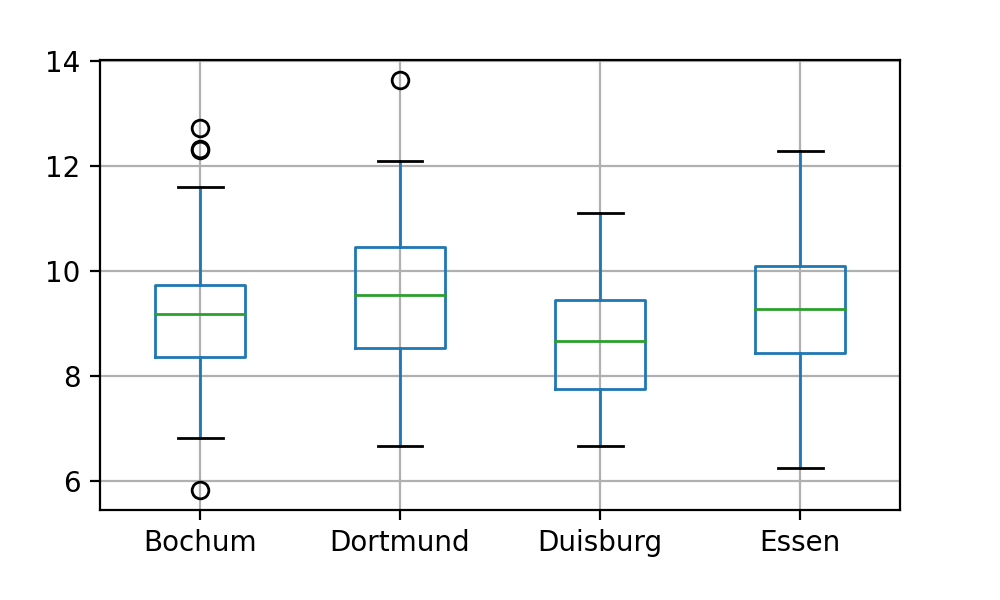
\includegraphics[width=0.66\textwidth]{./images/boxplot}
  \caption{Boxplots for rental prices in €/m²}
  \label{fig:boxplots}
\end{figure}

\subsection{Requirements for ANOVA}

As described in the methods part. To conduct an ANOVA a few requirements have to be fulfilled. First, the individual datapoints have to be sampled independent from each other. We can assume that this is the case since there are thousands of listings on Immobilienscout24 and just a few of them have been randomly sampled into our dataset. There are no signs of dependence between the different properties contained in the dataset.
Secondly the ANOVA requires equal variance within each of the 4 groups.

\begin{table}[ht]
  \centering
  \captionabove{Variances within the 4 cities}
  \label{tab:variances}
  \begin{tabular}{c|cccc}
    Rental Price        & $Dortmund$ & $Duisburg$ & $Bochum$ & $Essen$ \\
    \hline
    variance in (€/m²)² & 1.84       & 1.30       & 1.76     & 1.41    \\
  \end{tabular}
\end{table}

As visible in Table \ref{tab:variances} the maximum difference in variances between any two cities does not even exceed a factor of 1.5. Also the interquartile ranges in Figure~\ref{fig:boxplots} suggest, that the variance does not differ too much between cities.
The next requirement of an ANOVA is, that the values within each group shall be apoximately normal distributed. Figure ~\ref{fig:qqplots} shows Quantile-Quantile plots for each of the four cities. For this the sample data has been z-standardized, to be rougly in the same range as the quantiles of the normal distribution. Points that fall onto the 45-degree line running through each Q-Q plot signify that the quantile there is the same in the standardized sample data as in a standard normal distribution.
We can see, that most points stay relatively close to the straight line, signifying that the data in each city is apoximately normal distributed. Especially Bochum shows some minor deviations though, when it comes to the higher quantiles.
We will check this off as close enough to be able to conduct an analysis of variance.

\begin{figure}[h]
  \centering
  \begin{subfigure}[b]{0.40\textwidth}
    \centering
    
\includegraphics[width=\textwidth]{./images/qqplot-Dortmundc}
    \caption{Q-Q plot Dortmund}
    \label{fig:qqplot-Dortmund}
  \end{subfigure}
  \begin{subfigure}[b]{0.40\textwidth}
    \centering
    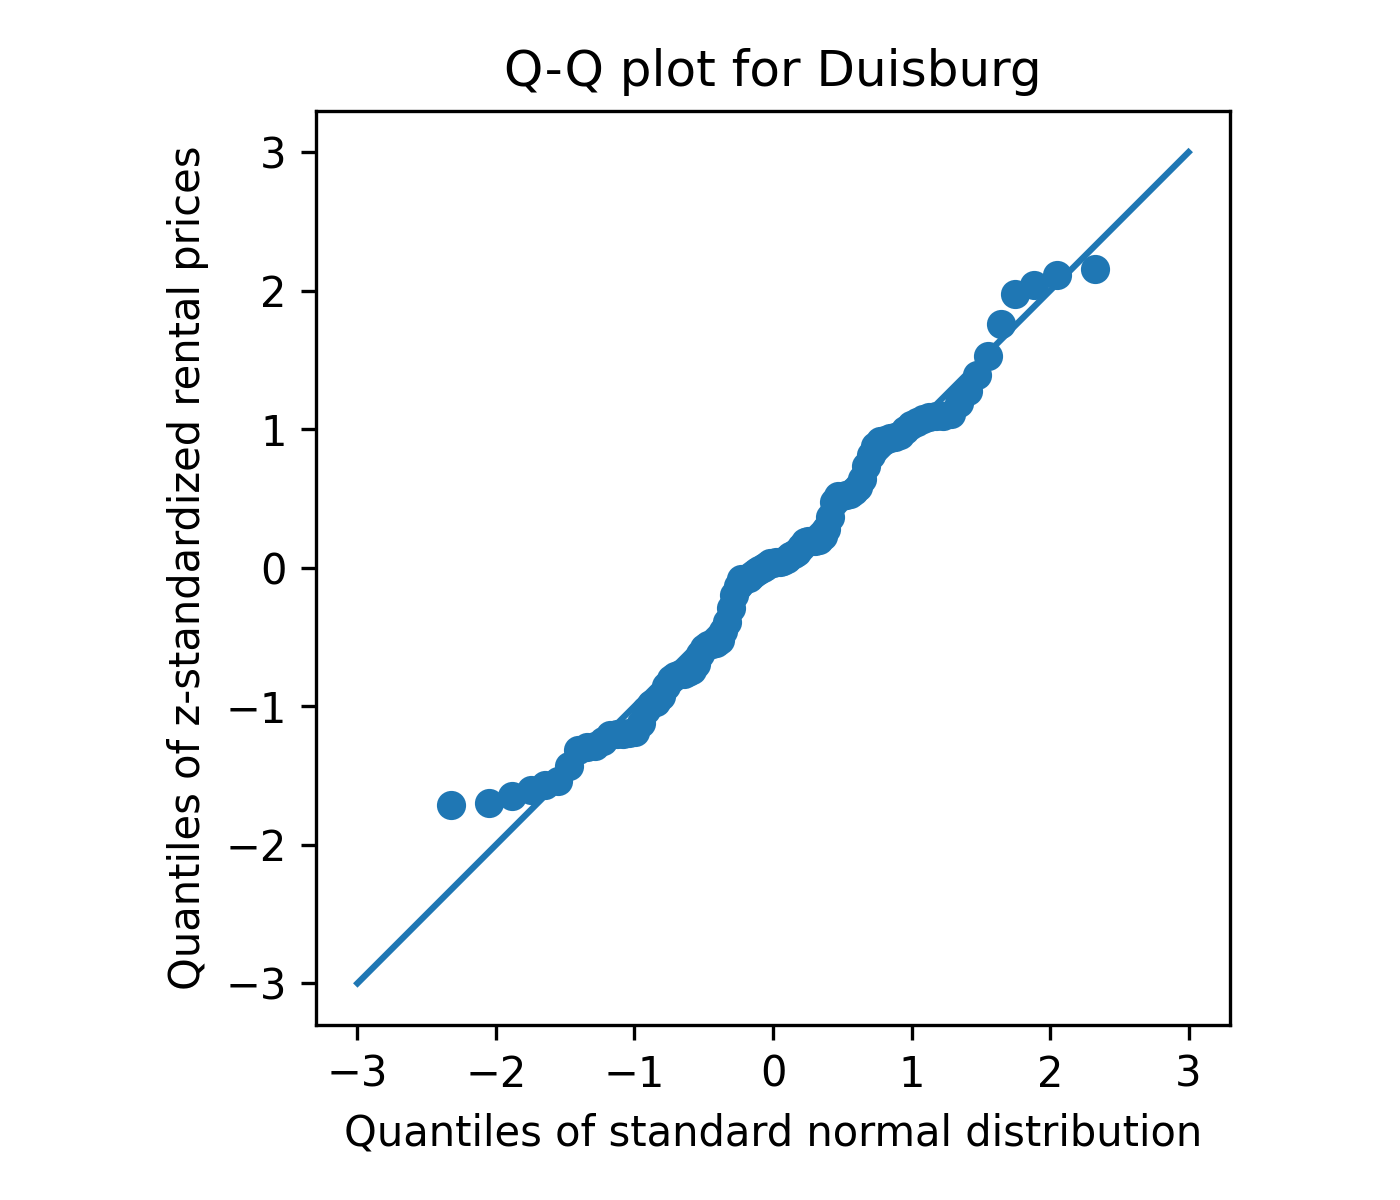
\includegraphics[width=\textwidth]{./images/qqplot-Duisburgc}
    \caption{Q-Q plot Duisburg}
    \label{fig:qqplot-Duisburg}
  \end{subfigure}
  \begin{subfigure}[b]{0.40\textwidth}
    \centering
    
\includegraphics[width=\textwidth]{./images/qqplot-Bochumc}
    \caption{Q-Q plot Bochum}
    \label{fig:qqplot-Bochum}
  \end{subfigure}
  \begin{subfigure}[b]{0.40\textwidth}
    \centering
    
\includegraphics[width=\textwidth]{./images/qqplot-Essenc}
    \caption{Q-Q plot Essen}
    \label{fig:qqplot-Essen}
  \end{subfigure}

  \caption{Q-Q plots to compare distribution of values within cities with the standard normal distribution }
  \label{fig:qqplots}
\end{figure}

\subsection{ANOVA for all 4 groups}


To conduct an ANOVA for the 4 cities, suqare sums (between and within) have been calculated like displayed in Table \ref{tab:anova1}, resulting in an F test statisic of $F = 4.6811 $. We will consider an alpha-level of $\alpha = 0.05 $ for this test.
The hypotheses for the ANOVA are as follows:
\[ H_0: \forall c_1,c_2 \in \{Dortmund,Duisburg,Bochum,Essen\}: \ \mu_{c_1} = \mu_{c_2}   \]
\[ H_1: \exists c_1,c_2 \in \{Dortmund,Duisburg,Bochum,Essen\}: \ \mu_{c_1} \neq \mu_{c_2}   \]
The cumulative distribution function of an F distribution with $df_1 = 3$ and $df_2 = 196$ yields: $ p = 1 - F_{3,196}(4.6811) = 0.0035$.
So if the probability of getting $ F \ge  4.6811$ is only 0.35\% in case the null hypothesis, that all cities have the same rental price mean, is true.
The critical value $F_{crit}$ can be retrieved as the $1-\alpha$-quantile of an $F_{3,196}$ distribution, which results in $F_{crit} = 2.6506$.
Our $p-value = 0.0035$ is less than $\alpha = 0.05$, therefore we reject the null hypothesis and conclude that there are significant differences between the mean rental prices of the cities Dortmund, Duisburg, Bochum and Essen. However this does not tell us, which two particular cities differ from one another in their mean.

\begin{table}[ht]
  \centering
  \captionabove{ANOVA to detect, if mean rental price differs between cities}
  \label{tab:anova1}
  \begin{tabular}{l|llll}
    Source of variation      & square sum & df  & mean square sum & F     \\
    \hline
    between cities           & 22.145     & 3   & 7.382           & 4.681 \\
    within cities (residual) & 309.078    & 196 & 1.577           &       \\
    total                    & 331.223    & 199 &                 &       \\
  \end{tabular}
\end{table}

\subsection{Pairwise Differences between cities}

To test whether the mean rental price differs between two particular cities, we can also conduct a couple of one-way ANOVAs with just two groups each. To cover all combinations of cities, $ 4\choose2 = \frac{4!}{2! * 2!} = 6 $ tests have to be made. Typically a two sample t-test is used for the comparison of two group means, but since the method one-way ANOVA has already been introduced and yields the same results, it is also feasible. For example the hypotheses for the pairwise comparison between Dortmund and Bochum would be:
\[ H_0: \mu_{Dortmund} = \mu_{Bochum} \ \ \ \ \ H_1: \mu_{Dortmund} \neq \mu_{Bochum}  \]
As each ANOVA processes 100 data points in total, distributed equally to 2 groups, under the assumption that the mean rental price does not differ between the cities, the test statistic F would follow an $F_{1,98}$ distribution. So we can easibly calculate the critical F value $F_{crit}$ again as the $1-\alpha$-quantile of an $F_{1,98}$ distribution. For $\alpha = 0.05$ this results in $F_{crit} = 3.9381$ for every of the 6 ANOVAs. As we want to make use of bonferroni correction to adress the multiple testing problem, we want to set $\alpha = \frac{0.05}{6} = 0.0083$, which would then result in $F_{crit} = 7.2515$, a higher hurdle for our test statistic to overcome.
Table \ref{tab:anova2} shows the outcome of these ANOVAs.

\begin{table}[ht]
  \centering
  \captionabove{ANOVA to detect, if mean rental price differs between cities}
  \label{tab:anova2}
  \begin{tabular}{l|llllll}
    City-Pair           & $SS_{between}$ & $SS_{within}$ & $MQS_{between}$ & $MQS_{within}$ & $F$    & $p$    \\
    \hline
    Dortmund - Duisburg & 20.455         & 153.876       & 20.455          & 1.57           & 13.027 & 0.0005 \\
    Dortmund - Bochum   & 3.522          & 176.124       & 3.522           & 1.797          & 1.959  & 0.1647 \\
    Dortmund - Essen    & 1.29           & 159.202       & 1.29            & 1.625          & 0.794  & 0.3751 \\
    Duisburg - Bochum   & 7.002          & 149.876       & 7.002           & 1.529          & 4.578  & 0.0349 \\
    Duisburg - Essen    & 11.473         & 132.953       & 11.473          & 1.357          & 8.457  & 0.0045 \\
    Bochum - Essen      & 0.549          & 155.201       & 0.549           & 1.584          & 0.347  & 0.5573 \\
  \end{tabular}
\end{table}

Close attention should be paid here to the $F$ and $p$ values. Under $\alpha = 0.05$ three pairwise tests, result in rejecting the null hypothesis. For the comparisons Dortmund vs. Duisburg ($p = 0.0005$), Duisburg vs. Bochum ($p = 0.0349$) and Duisburg vs. Essen ($p = 0.0045$) the p value is less than 0.05 and the F value surpasses $F_{crit} = 3.9381$. This means, for those comparisons we would say that the rental price means are probably different. However, it is well possible that the difference between Duisburg and Bochum just stems from random variance: It would be a mistake to interpret the result with an uncorrected alpha-level of $\alpha = 0.05$. Applying our bonferroni-corrected $\alpha = 0.0083$ reveals that actually only the differences in Dortmund vs. Duisburg and Duisburg vs. Essen can be classified as significant effects. In this way, we can confidently say, that Duisburg has significantly significantly lower rental prices than Dortmund and it also has significantly lower prices than Essen. No significant difference can be concluded for all other pairs of cities.

\section{Summary}

The goal of this project was to find out how the rental prices differ between the 4 largest cities in the ruhr area: Dortmund, Duisburg, Bochum and Essen. To answer this question data from Kaggle \citep{kaggle} was used, that consisted of the rental price per square meter for 200 properties that were listed on the online real estate portal Immobilienscout24. The data was sampled in such a way, that 50 properties could be assigned to each city. It has to be mentioned that it is hard to asess the quality of this data, as it might be only representing a small percentage of the properties that are up for rent.
We found that the overall mean for the rental price in the 4 cities of the ruhr area is  9.15 ($\pm 1.29$) €/m² while the sample mean differs between Dortmund (9.53 €/m²), Duisburg (8.62 €/m²), Bochum (9.15 €/m²) and Essen (9.30 €/m²).
To see if this difference is substantial or only caused by random variation a one-way ANOVA was calculated. Under the significance level $\alpha = 0.05$, we rejected the null hypothesis that the mean rental price does not differ between cities. Because this did not give us insight, which cities differ from another significantly in their rental prices, for each pair of two cities a separate one-way ANOVA was calculated. The 6 two-group ANOVAs used for this were bonferroni-corrected in their $\alpha$-level to $\alpha = \frac{0.05}{6} = 0.0083$. Here we found in 2 of the 6 tests that Duisburg had significantly lower rental prices than Dortmund and Essen. The other comparisons turned out to be not significant under $\alpha = 0.0083$.
This could lead to the conclusion, that it is cheaper to live in Duisburg than to live in Dortmund or Essen. However the reasons for this difference stay hidden. While location, local industry, living standard and popularity could be reasons for the difference in rental prices here, also potential biases should be kept in mind. For example it could be that the clients of Immobilienscout24 are not the same for Dortmund and Duisburg. If a big real estate firm puts a lot of modernized properties on the platform in one city while a real estate firm in another city chooses a different way to find tenants, this can result in bad representativity of the data. Also the non-significant effects found could turn out to be significant if our testing had more power. This could be achieved by more properties in the underlying dataset, such that the stardard error of means shrinks. Therefore interpretations of both, significant and non-significant results should be validated by more data in the future. Also a regression analysis taking into account other factors like property-size, floor of building, proximity to the city center, year of last renovation and other relevant variables would help to better understand the current real estate market in the ruhr area. It is also sensable that the prices fluctuate throughout the year, perhaps even in different cycles in different cities. When a place is closely bound to summer tourism, rent is likely higher in the summer than in the winter there. On the other hand cities with a good proportion of university students might experience spikes in rental prices as the demand rises with the start of a new semester.
Also it would be better to sample data from even more cities of germany, not just the ruhr area to help putting the prices in Dortmund, Duisburg, Essen and Bochum into context. But the more cities we add, the less likely it will be to find significant differences between two particular cities as the number of bonferroni-corrected tests would increase quadratically and lower the corrected $\alpha$-level by a lot.
In summary we do not think the differences in rental price are big enough to really influence practical living decisions in peoples everyday lives. We found significant differences but as Table \ref{tab:anova1} shows the variation within cities is still more than 14 times higher than the variation between cities, making the city alone a quite weak predictor of the rental price of a randomly chosen property.


\newpage
\addcontentsline{toc}{section}{Bibliography}
\renewcommand\refname{Bibliography}
\bibliographystyle{plainnat}
\bibliography{references}

\newpage
\appendix
\addsec{Appendix}
\subsection*{A \ Additional figures}
\addcontentsline{toc}{subsection}{A \hspace*{0.15cm} Additional figures}
\end{document}
